\documentclass[../main.tex]{subfiles}
\graphicspath{{\subfix{../images/}}}
\begin{document}


\section{Binomial expansion}
In your formula sheet you will see this on the first page:
\begin{figure}[h]
    \centering
    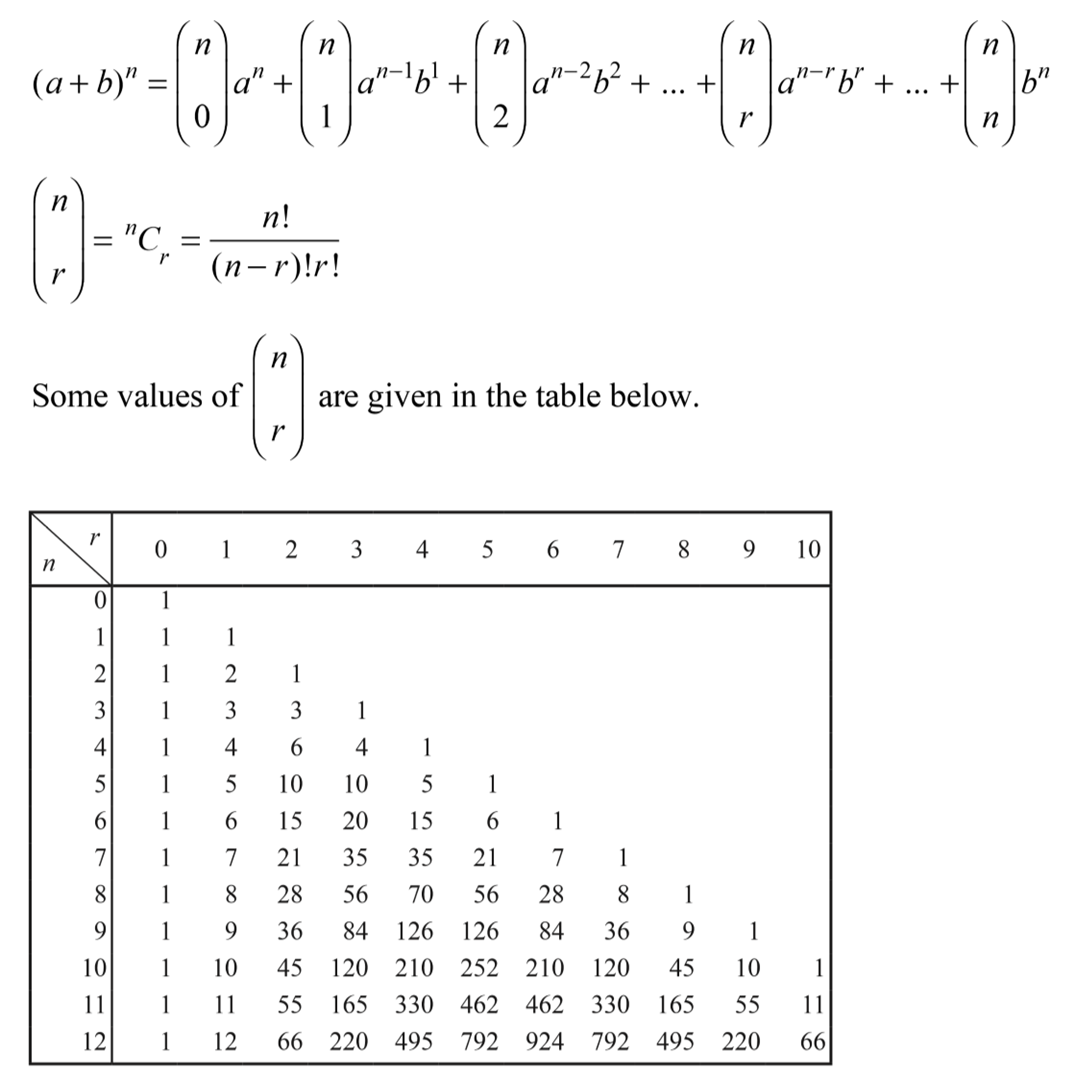
\includegraphics[width=0.75\linewidth]{images/binomial.png}
\end{figure}

This helps us expand out brackets that are raised to a high power.
The numbers in the table give the coefficients of the terms when we expand the brackets.
For example:
\[(a + b)^4 = a^4 + 4a^3 b + 6a^2 b^2 + 4a b^3 + b^4\]

Notice how the coefficients match the numbers in row 4 in the table.

Also notice that the powers start at 4 for the first term in the brackets and zero for the second term. They then decrease and increase by 1 each term respectively.

In general, the sum of the powers in each term will add to the power we are raising the bracket to (in the example this is 4).

Another example:
\begin{equation*}
\begin{split}
    (2a - 3b)^4 &= (2a)^4 + 4(2a)^3 (-3b) + 6(2a)^2 (-3b)^2 + 4(2a)(-3b)^3 + (-3b)^4 \\
&= 16a^4 -96a^3 b + 216a^2 b^2 - 216ab^3 + 81b^4
\end{split}
\end{equation*}

\pagebreak

\subsection*{Questions}
\label{Binomial Expansion}
Expand the following:

\begin{enumerate}
    \item \( (x+y)^3 \)
    \item \( (2x+y)^4 \)
    \item \( (2x-3)^5 \)
    \item \( (3x+2y)^4 \)
    \item \( (2x + \frac{1}{x^2 } )^4 \)
\end{enumerate}

Scholarship questions would tend to look more like this:

\begin{enumerate}
    \setcounter{enumi}{5}
    \item Find the term independent of \( x \) in \( (3x^2 - \frac{1}{3x})^{12}  \)
    \item Find the coefficient of the \( x^2 \) term in \( (x^2 + \frac{1}{x})^{10} \)
    \item Find the term independent of \( x \) in \( 2x^2 - \frac{3}{x})^6 \)
    \item It can be shown that \( \cos(\theta) = \frac{e^{i\theta}+e^{-i\theta}}{2}\) and that \( \sin(\theta) = \frac{e^{i\theta}-e^{-i\theta}}{2i}\)
    \item 
    Use these identities, or otherwise, to show that:

    \( \cos^6(\theta) = \frac{1}{32}\cos(6\theta) + \frac{3}{16}\cos(4\theta)+\frac{15}{32}\cos(2\theta)+\frac{5}{16}\)
\end{enumerate}




\end{document}